\subsection{Web of Trust}\label{sec:binding_keys_to_parties:wot}

The \gls{wot} is a cumulative, decentralized, and transitive trust model where anyone can verify and endorse the association between public keys and parties --- similarly to a reputation system. The \gls{wot} enables a decentralized network of trust to grow organically, relying on overlapping trust relationships rather than centralized parties. 

\remarkBlock{Certificates in \gls{wot}}{The most widely adopted format for certificates in \gls{wot} is the \gls{pgp} certificate format --- see \url{https://www.ietf.org/archive/id/draft-bre-openpgp-samples-01.html}.}

\remarkBlock{Indirect trust in the \gls{wot}}{Being a transitive trust model, in the \gls{wot} a party \texttt{A} may trust another party \texttt{C} either directly --- by issuing a \gls{pgp}-formatted digital certificate for the key pair of the party \texttt{C} as normally --- or indirectly. In the latter case, the party \texttt{A} trusts the party \texttt{C} if there exists a chain of trust between the party \texttt{A} and the party \texttt{C}. In other words, trust in one party extends to others parties based on a chain of endorsements. For example, if the party \texttt{A} directly trusts a party \texttt{B}, and the party \textbf{B} directly trusts the party \texttt{C}, then the party \texttt{A} indirectly trusts the party \texttt{C} --- even without direct interaction between the party \texttt{A} and the party \texttt{C}. Intuitively, parties can set thresholds on the length of the chain of trust they accept.}

A comparison between \gls{pki} and \gls{wot} is provided in \Cref{figure:pki_vs_wot}

\subsubsection{Pretty Good Privacy}\label{sec:binding_keys_to_parties:wot:pgp}

\gls{pgp} is both a suite of cryptographic ciphers (mainly for encryption and creation of digital signatures) and the name of their original implementation by Phil Zimmermann\footnote{\url{https://philzimmermann.com/}}) in 1991. \gls{pgp} was later standardized as OpenPGP \cite{rfc9580} --- see \url{https://www.openpgp.org/} --- and its reference implementation is GnuPG --- see \url{https://gnupg.org}. OpenPGP is the main standard supporting \gls{wot} --- from another point of view, \gls{wot} is the trust model used in OpenPGP to establish and manage trust.

\warningBlock{On the (in)security of \gls{pgp}}{Some deem \gls{pgp} to be outdated, badly designed, and with serious vulnerabilities --- see \url{https://latacora.micro.blog/2019/07/16/the-pgp-problem.html} and \url{https://blog.cryptographyengineering.com/2014/08/13/whats-matter-with-pgp/}.}

\begin{figure}[t!]
	\begin{center}
		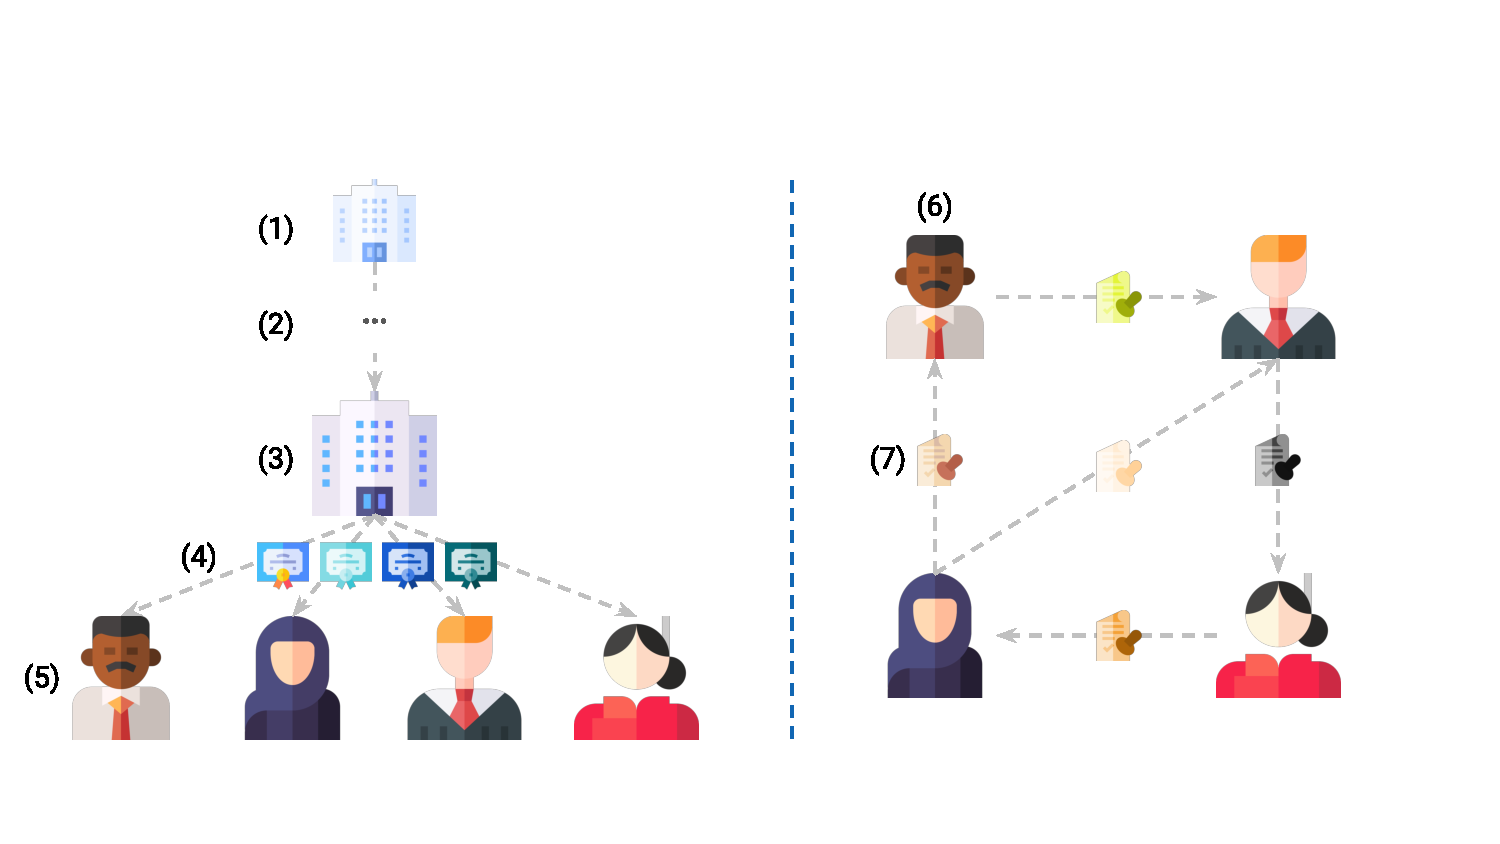
\includegraphics[trim={0cm 2cm 2.5cm 3cm},clip,width=0.75\linewidth]{resources/pdf/pki_vs_wot.pdf}
		\caption{\gls{pki} vs. \gls{wot}. In a \gls{pki}, one or more root \glspl{ca} (1) issue X.509-formatted digital certificates to other \glspl{ca}. Subordinate \glspl{ca} (3) issue digital certificates (4) only to parties (5) --- a party may represent an entire organization, a part of an organization, or, seldom, a single user. Between root \gls{ca} and subordinate \glspl{ca}, there may be zero or more intermediate \glspl{ca} (2). The key pairs of an intermediate \gls{ca} are endorsed by root or other intermediate \glspl{ca}. Usually, an intermediate \gls{ca} issues digital certificates only to intermediate or subordinate \glspl{ca} and not to parties. Conversely, in \gls{wot} a party (6) receives \gls{pgp}-formatted digital certificates by other parties.}
		\label{figure:pki_vs_wot}
	\end{center}
\end{figure}
